\documentclass{article}

\setlength\parindent{0pt}

\title{Assignment 2}
\date{\vspace{-5ex}}

\usepackage{tikz,pgfplots}
\usepackage{amsmath}
\usepackage{amssymb}
\usepackage{epstopdf}
\usepackage{mathtools}
\usepackage{calculator}
\usepackage{a4wide}
\pgfplotsset{compat=1.12}

\usepackage{Sweave}
\begin{document}
\input{HW2_Ex_1-5_V02-concordance}

\textbf{Exercise 1} \\

\textbf{\textit{Part A - Geometric Brownian Motion}} \\

Suppose we have process X following geometric Brownian motion dynamics with drift $\mu = 0.1$, $\sigma = 0.1$. By using the random walk approximation as well as the Cholesky decomposition to generate Brownian motion, simulate $1000$ paths for the time interval $[0,1]$. In your computations use $n = 250$ equidistant time discritization points with $t0 = 0$ and $tn = T = 1$. Compare the computation times
corresponding to the two method. 

\begin{Schunk}
\begin{Sinput}
> #Function Random Walk Approximation
> GBM <- function(S0, mu, sigma){
+   set.seed(1000)
+   t <- seq(0, 1, 1/250)
+   St_vec <- matrix(S0, 251, 1000)
+   for(i in 1:1000){
+     Z1 <- rnorm(250, 0, 1)
+     for(j in 1:250){
+       St_vec[j+1, i] <- St_vec[j,i] * exp((mu-1/2*sigma^2)*(t[j+1]-t[j]) + sigma * sqrt(t[j+1]-t[j]) * Z1[j])
+     }
+   }
+   plot(St_vec[,1], type="l", ylim=c(0, 150))
+   for(i in 2:1000){
+     lines(St_vec[,i], type="l")
+   }
+ }
> #Function Cholesky Approach
> GBM_COL <- function(S0, mu, sigma){
+   set.seed(1000)
+   t <- seq(0, 1, 1/250)
+   A <- matrix(0, 250, 250)
+   index <- 0
+   for(j in 1:250){
+     index <- index + 1
+     for(i in index:250){
+       A[i,j] <- sqrt(t[i+1]-t[i])
+     }
+   }
+   St_vec <- matrix(S0, 250, 1000)
+   for(i in 1:1000){
+     Z2 <- rnorm(250, 0, 1)
+     W <- A %*% Z2
+     St_vec[,i] <- S0 * exp((mu-1/2*sigma^2)*(t[j+1]-t[j]) + sigma * W)
+   }
+   plot(St_vec[,1], type="l", ylim=c(0, 150))
+   for(i in 2:1000){
+     lines(St_vec[,i], type="l")
+   }
+ }
\end{Sinput}
\end{Schunk}

\begin{Schunk}
\begin{Sinput}
> #Chosen Value for S0 = 50
> #mu=0.1, sigma=0.1
> par(mfrow=c(2,1))
> GBM(50, 0.1, 0.1)
> GBM_COL(50, 0.1, 0.1)
\end{Sinput}
\end{Schunk}
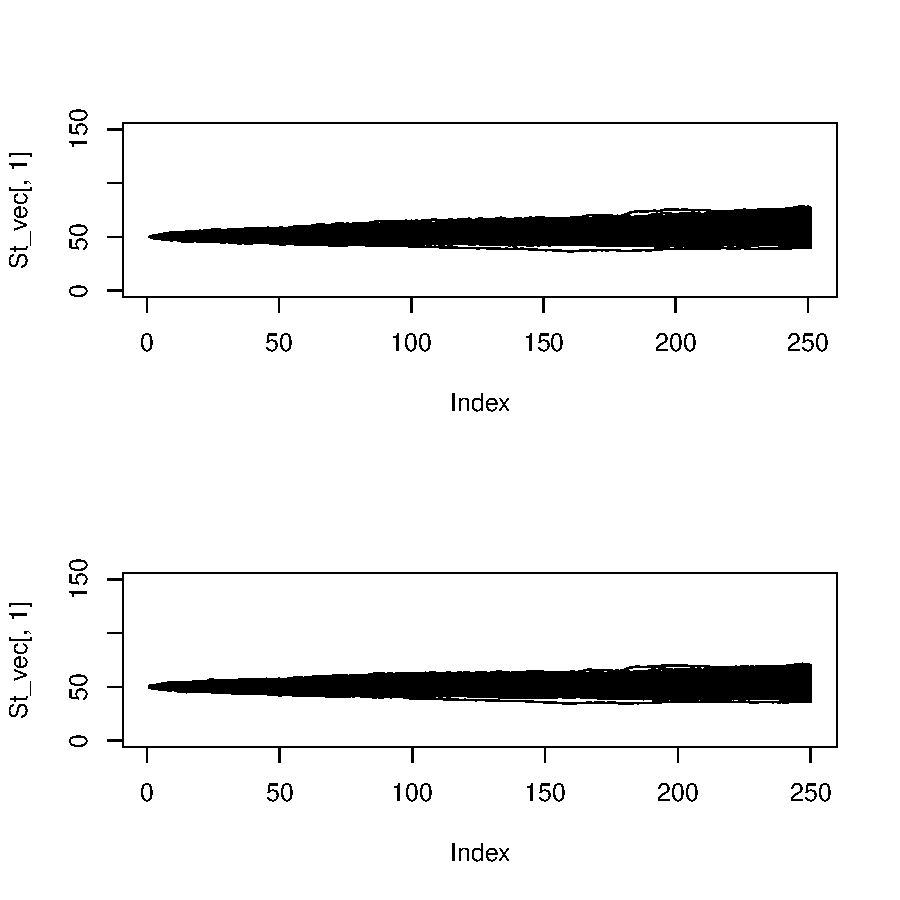
\includegraphics{HW2_Ex_1-5_V02-002}


Repeat this exercise for $\mu = 0.4$, $\sigma = 0.4$. (keep
the seed fixed in order to see the impact of different parameters). For all cases provide a plot with the simulated paths.

\begin{Schunk}
\begin{Sinput}
> #Chosen Value for S0 = 50
> #mu=0.4, sigma=0.4
> par(mfrow=c(2,1))
> GBM(50, 0.4, 0.4)
> GBM_COL(50, 0.4, 0.4)
\end{Sinput}
\end{Schunk}
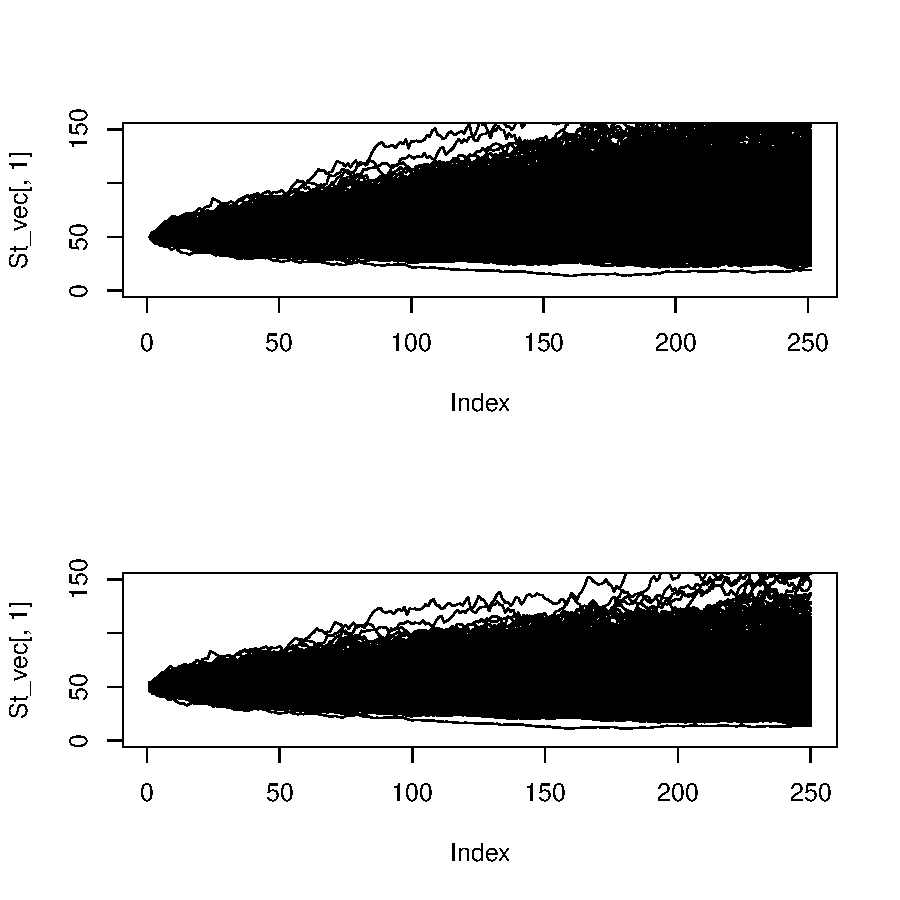
\includegraphics{HW2_Ex_1-5_V02-003}


\textbf{\textit{Part B - Poisson Process}} \\

Simulate 50 paths for a Poisson process with parameter $\lambda = 2$. Now keep the seed fixed and take $\lambda = 0.5$. For both cases provide a plot with the simulated paths.

\begin{Schunk}
\begin{Sinput}
> sim.Poiss <- function(lambda, n, T.stop, X =list()) {
+   for (i in 1:n) {
+     t <- 0
+     I <- 0
+     S <- c()
+     u <- runif(n = 1, 0, 1)
+     t <- t - log(u)/lambda
+     
+     while (t < T.stop) {
+       I <- I + 1
+       S[I] <- t
+       u <- runif(1, 0, 1)
+       t <- t-log(u)/lambda
+     }
+     X[[i]] <- c(0, S)
+     X[[i]] <- X[[i]][1:150]
+   }
+   Poiss <- do.call("cbind", X)
+ } 
> # inputs
> T.stop <- 500
> n <- 50
> lambda.1 <- 2
> lambda.2 <- 0.5
> # simulations
> set.seed(2019)
> draws.1 <- sim.Poiss(lambda.1, n, T.stop)
> set.seed(2019)
> draws.2 <- sim.Poiss(lambda.2, n, T.stop)
> # plotting
> par(mfrow=c(2,1))
> matplot(x = draws.1, y = 0:149, type = "s", col = "darkcyan",
+         xlim = c(0, 50), xlab = "time", ylab = "N(t)",
+         main = "Poisson Process paths (lambda = 2)")
> matplot(x = draws.2, y = 0:149, type = "s", col = "darkcyan",
+         xlim = c(0, 50), xlab = "time", ylab = "N(t)",
+         main = "Poisson Process paths (lambda = 0.5)")
\end{Sinput}
\end{Schunk}


\newpage
\textbf{Exercise 2} \\
Suppose we want to price a European call option written on a stock with initial value $S_0 = 80, \sigma = 0.2, \mu = 0.2$. The maturity of the option is in $T = 1$ year and the strike price is $K = 100$. The risk-free interest rate is $r = 2\%$.\\
First, we price the option analytically by using the closed-form price Black-Scholes formula. Second, we price it numerically by using naive Monte Carlo (with $n = 10000$ paths) and additionally compute the corresponding Monte Carlo standard error and confidence interval for $\alpha = 0.05$.
\begin{Schunk}
\begin{Sinput}
> set.seed(1)
> # given
> S0 <- 80
> K <- 100
> vol <- 0.2
> T_years <- 1
> r <- 0.02
> ## Analytically (by use of closed-form price BS-formula)
> d.1 <- (log(S0/K) + (r+vol^2/2)*T_years) / vol*sqrt(T_years)
> d.2 <- d.1 - vol*sqrt(T_years)
> Call.price <- S0*pnorm(d.1) - exp(-r*T_years)*K*pnorm(d.2)
> Call.price
\end{Sinput}
\begin{Soutput}
[1] 1.427365
\end{Soutput}
\begin{Sinput}
> ## naive MC Call Option Pricing
> Call.naive.mc <- function(S0, K, vol, T_years, r, n, alpha) {
+   Z <- rnorm(n)
+   ST.est <- S0*exp((r-vol^2/2)*T_years + vol*sqrt(T_years)*Z) # Simulate ST values (GBM)
+   payoff <- exp(-r*T_years)*pmax(ST.est-K, 0) # payoffs 
+   
+   Price <- mean(payoff)  # naive MC estimate
+   se <- sd(payoff)/sqrt(n)
+   z.score <- qnorm(1-alpha/2, mean = 0, sd = 1)
+   low.b <- Price - z.score*se
+   up.b <- Price + z.score*se
+   width <- up.b - low.b
+   return(c(MC.naive=Price, s.e.=se, Lower=low.b, Upper=up.b, ci.width = width))
+ }
> # given
> n <- 10000
> alpha <- 0.05
> Call.naive.mc(S0, K, vol, T_years, r, n, alpha)
\end{Sinput}
\begin{Soutput}
  MC.naive       s.e.      Lower      Upper   ci.width 
1.45657787 0.05092886 1.35675914 1.55639660 0.19963746 
\end{Soutput}
\end{Schunk}

\newpage
\textbf{Exercise 3} \\

Suppose we want to price a European call option written on a stock with initial value $S0 = 80$, $\sigma = 0.2$. The maturity of the option is in $T = 1$ year and the strike price is $K = 80$. Assume that the risk-free interest rate is $r = 2\%$. Price the option with antithetic variates (simulate n = 10000 paths). Estimate the reduction in
the variance relative to naive Monte Carlo.\\

\begin{Schunk}
\begin{Sinput}
> # given
> S0 <- 80
> K <- 80
> vol <- 0.2
> T_years <- 1
> r <- 0.02
> #Antithetic Variates
> Call.anti.var <- function(S0, K, vol, T_years, r, n, alpha){
+   Z <- rnorm(n/2)
+   ST.est <- S0*exp((r-vol^2/2)*T_years + vol*sqrt(T_years)*(Z)) # Simulate ST values (GBM)
+   payoff <- exp(-r*T_years)*pmax(ST.est-K, 0) # payoffs
+   Price <- mean(payoff) 
+   se <- sd(payoff)/sqrt(n)
+   z.score <- qnorm(1-alpha/2, mean = 0, sd = 1)
+   low.b <- Price - z.score*se
+   up.b <- Price + z.score*se
+   width <- up.b - low.b
+   return(c(Anti.Var=Price, s.e.=se, Lower=low.b, Upper=up.b, ci.width = width))
+ }
> # given
> n <- 10000
> alpha <- 0.05
> #Analytical
> d.1 <- (log(S0/K) + (r+vol^2/2)*T_years) / vol*sqrt(T_years)
> d.2 <- d.1 - vol*sqrt(T_years)
> Call.price <- S0*pnorm(d.1) - exp(-r*T_years)*K*pnorm(d.2)
> Call.price
\end{Sinput}
\begin{Soutput}
[1] 7.13283
\end{Soutput}
\begin{Sinput}
> #Simulation
> Call.naive.mc(S0, K, vol, T_years, r, n, alpha)
\end{Sinput}
\begin{Soutput}
 MC.naive      s.e.     Lower     Upper  ci.width 
7.0336091 0.1108705 6.8163070 7.2509113 0.4346043 
\end{Soutput}
\begin{Sinput}
> Call.anti.var(S0, K, vol, T_years, r, n, alpha)
\end{Sinput}
\begin{Soutput}
 Anti.Var      s.e.     Lower     Upper  ci.width 
7.2982441 0.1106325 7.0814083 7.5150798 0.4336715 
\end{Soutput}
\end{Schunk}

The reduction in variance is very small as our european call option is at the money (K=S=80). This means that we apply the antithetic variates method to the non-increasing part of a call-payoff-function.\\

Now take the strike value K = 40 (option is deep-in-the-money) and redo your computations (keep the seed fixed).
How is the reduction in variance affected?

\begin{Schunk}
\begin{Sinput}
> K <- 40
> n <- 10000
> alpha <- 0.05
> #Analytical
> d.1 <- (log(S0/K) + (r+vol^2/2)*T_years) / vol*sqrt(T_years)
> d.2 <- d.1 - vol*sqrt(T_years)
> Call.price <- S0*pnorm(d.1) - exp(-r*T_years)*K*pnorm(d.2)
> Call.price
\end{Sinput}
\begin{Soutput}
[1] 40.79255
\end{Soutput}
\begin{Sinput}
> #Simulation
> Call.naive.mc(S0, K, vol, T_years, r, n, alpha)
\end{Sinput}
\begin{Soutput}
  MC.naive       s.e.      Lower      Upper   ci.width 
40.8625021  0.1638280 40.5414052 41.1835990  0.6421938 
\end{Soutput}
\begin{Sinput}
> Call.anti.var(S0, K, vol, T_years, r, n, alpha)
\end{Sinput}
\begin{Soutput}
  Anti.Var       s.e.      Lower      Upper   ci.width 
40.3556679  0.1590723 40.0438918 40.6674439  0.6235521 
\end{Soutput}
\end{Schunk}

As we are now in the money $(S>K)$, the variance decreases to a higher extent since we apply the method to the increasing and monotone part of the call-payoff-function.

\newpage
\textbf{Exercise 4} \\
Suppose we want to estimate $\theta = E((1-X^2)^{1/2})$, $X \sim U(0,1)$. \\

\textbf{a)} Computing naive Monte Carlo estimator of $\theta$ as well as the confidence interval for $\alpha = 0.05$ by taking $n = 10000$. 
\begin{Schunk}
\begin{Sinput}
> set.seed(2019)
> # Naive MC-algorithm
> mc <- function(f, ndraws, alpha) {
+   draws <- runif(n = ndraws, 0, 1)
+   theta <- mean(f(draws))
+   se <- sd(f(draws))/sqrt(ndraws)
+   z.score <- qnorm(1-alpha/2, mean = 0, sd = 1)
+   low.b <- theta - z.score*se
+   up.b <- theta + z.score*se
+   width <- up.b - low.b
+   return(c(MC.naive=theta, s.e.=se, Lower=low.b, Upper=up.b, ci.width = width))
+ }
> f <- function(x) (sqrt(1-x^2)) # given function
> ndraws <- 10000 # number of draws
> alpha <- 0.05 # alpha 
> MC.naive <- mc(f, ndraws, alpha); MC.naive
\end{Sinput}
\begin{Soutput}
   MC.naive        s.e.       Lower       Upper    ci.width 
0.789296626 0.002214547 0.784956194 0.793637059 0.008680866 
\end{Soutput}
\end{Schunk}


\textbf{b)} \\
The ratio of the variance of the optimally controlled estimator to that of the uncontrolled estimator is given by
$$ \frac{Var(X+c^*(Y-E(Y)))}{Var(X)} = \frac{Var(X)-\frac{Cov(X,Y)^2}{Var(Y)}}{Var(X)} = 1 - \rho(X,Y)^2 $$
Thus, the effectiveness of a control variate, as measured by the variance reduction ratio is determined by the strength of the correlation between the quantity of interest $X$ and the control $Y$. The sign of the correlation is irrelevant because it is absorbed in the optimal coefficient $c^*$. Therefore, the higher the correlation the better the control variant (ceteris paribus).
\begin{Schunk}
\begin{Sinput}
> set.seed(2019)
> u <- runif(n = ndraws, 0, 1)
> X <- sqrt(1-u^2)
> Y.1 <- u
> Y.2 <- u^2
> cor(X, Y.1)
\end{Sinput}
\begin{Soutput}
[1] -0.9198958
\end{Soutput}
\begin{Sinput}
> cor(X, Y.2)
\end{Sinput}
\begin{Soutput}
[1] -0.9832095
\end{Soutput}
\end{Schunk}
As we can see $|\rho((1-X^2)^{1/2}, X^2)| > |\rho((1-X^2)^{1/2},X)|$, thus it is better to use $X^2$ instead of $X$ as a control variate. \\ 


\textbf{c)} \\
Now, using $X^2$ as a control variate we stimate $\theta$ and obtain the corresponding confidence intervals. For the pilot simulation we used $n = 1000$ to come up with optimal $c$ (in the code called $a$). For the main part of simulation we used $n = 10000$ samples. 
\begin{Schunk}
\begin{Sinput}
> set.seed(2019)
> mc.cv <- function(f, k, n, alpha) {
+   # pilot simulation
+   u1 <- runif(k)
+   X1 <- f(u1)
+   Y1 <- u1^2
+   a <- -cov(X1, Y1) / var(Y1) # estimate of c*
+ 
+   # main simulation
+   u <- runif(n)
+   X <- f(u)
+   Y <- u^2
+   
+   Z <- X + a * (Y - mean(Y))
+   theta <- mean(Z) # MC-CV-estimate
+   se <- sd(Z)/sqrt(n) 
+   z.score <- qnorm(1-alpha/2, mean = 0, sd = 1)
+   low.b <- theta - z.score*se
+   up.b <- theta + z.score*se
+   width <- up.b - low.b
+   return(c(MC.cv=theta, s.e.=se, Lower=low.b, Upper=up.b, ci.width = width))
+ }
> f <- function(x) (sqrt(1-x^2)) # given function
> k <- 1000 # draws pilot
> n <- 10000 # draws main
> alpha <- 0.05 # alpha 
> MC.CV <- mc.cv(f, k, n, alpha); MC.CV
\end{Sinput}
\begin{Soutput}
       MC.cv         s.e.        Lower        Upper     ci.width 
0.7882717198 0.0004101219 0.7874678956 0.7890755441 0.0016076485 
\end{Soutput}
\end{Schunk}


\textbf{d)} \\
Comparing these results shows that the method using the control variate performs better, as the standard error (s.e.), as well as the width of the confidence interval is smaller.
\begin{Schunk}
\begin{Sinput}
> MC.naive
\end{Sinput}
\begin{Soutput}
   MC.naive        s.e.       Lower       Upper    ci.width 
0.789296626 0.002214547 0.784956194 0.793637059 0.008680866 
\end{Soutput}
\begin{Sinput}
> MC.CV
\end{Sinput}
\begin{Soutput}
       MC.cv         s.e.        Lower        Upper     ci.width 
0.7882717198 0.0004101219 0.7874678956 0.7890755441 0.0016076485 
\end{Soutput}
\end{Schunk}



\newpage
\textbf{Exercise 5} \\
Recall we want to price a European call option written on a stock with initial value $S_0 = 80, \sigma = 0.2, \mu = 0.2$. The maturity of the option is in $T = 1$ year and the strike price is $K = 100$. The risk-free interest rate is $r = 2\%$.\\
We price the option by using the underlying stock as a control variate (with $n = 10000$) and compare the results to the analytical price. Furthermore, we compare it to the naive Monte Carlo, for which we also calculate the amount of the reduction in the variance.
\begin{Schunk}
\begin{Sinput}
> # given
> S0 <- 80
> K <- 100
> vol <- 0.2
> T_years <- 1
> r <- 0.02
> ## analytically (see Ex 2)
> Call.price
\end{Sinput}
\begin{Soutput}
[1] 40.79255
\end{Soutput}
\begin{Sinput}
> ## naive MC (see Ex 2)
> n <- 10000
> alpha <- 0.05
> set.seed(1)
> Call.naive.mc(S0, K, vol, T_years, r, n, alpha)
\end{Sinput}
\begin{Soutput}
  MC.naive       s.e.      Lower      Upper   ci.width 
1.45657787 0.05092886 1.35675914 1.55639660 0.19963746 
\end{Soutput}
\begin{Sinput}
> ## MC with control variates
> Call.mc.cv <- function(S0, K, vol, T_years, r, k, n, alpha) {
+   # pilot simulation
+   Z1 <- rnorm(k)
+   ST.est <- S0*exp((r-vol^2/2)*T_years + vol*sqrt(T_years)*Z1)  # Simulate ST values (GBM)
+   payoff <- exp(-r*T_years)*pmax(ST.est-K, 0) # payoffs 
+   a <- -cov(ST.est,payoff)/var(ST.est) # estimate of c*
+   
+   # main simulation
+   Z2 <- rnorm(n)
+   ST.est <- S0*exp((r-vol^2/2)*T_years + vol*sqrt(T_years)*Z2)  # Simulate ST values (GBM)
+   payoff <- exp(-r*T_years)*pmax(ST.est-K, 0) # payoffs 
+   
+   payoff_cv <- payoff + a*(ST.est - S0*exp(r*T_years))
+   Price <- mean(payoff_cv) # MC-CV-estimate
+   se <- sd(payoff_cv)/sqrt(n)
+   z.score <- qnorm(1-alpha/2, mean = 0, sd = 1)
+   low.b <- Price - z.score*se
+   up.b <- Price + z.score*se
+   width <- up.b - low.b
+   return(c(MC.cv=Price, s.e.=se, Lower=low.b, Upper=up.b, ci.width = width))
+ }
> # given
> k <- 10000
> n <- 10000
> alpha <- 0.05
> set.seed(1)
> Call.mc.cv(S0, K, vol, T_years, r, k, n, alpha)
\end{Sinput}
\begin{Soutput}
     MC.cv       s.e.      Lower      Upper   ci.width 
1.46006096 0.03954383 1.38255647 1.53756545 0.15500898 
\end{Soutput}
\begin{Sinput}
> ## Amount of reduction in the variance
> # Naive
> set.seed(1)
> var.naive <- (Call.naive.mc(S0, K, vol, T_years, r, n, alpha)["s.e."])^2
> names(var.naive) <- "Var"
> # Control variate
> set.seed(1)
> var.cv <- (Call.mc.cv(S0, K, vol, T_years, r, k, n, alpha)["s.e."])^2
> names(var.cv) <- "Var"
> # reduction
> reduc.abs <- var.naive - var.cv
> reduc.rel <- (var.naive - var.cv) / var.naive*100
> reduc <- c(reduc.abs, reduc.rel)
> reduc  <- round(reduc, digits = 6)
> names(reduc) <- c("Absolute Var reduction", "Relative Var reduction %")
> reduc
\end{Sinput}
\begin{Soutput}
  Absolute Var reduction Relative Var reduction % 
                 0.00103                 39.71217 
\end{Soutput}
\end{Schunk}
As we can see, pricing the option by using the underlying stock as a control variate comes closer to the analytical solution (not argued by the point estimate, but rather by judging the s.e. and confidence interval), compared to using naive MC. This fact is also indicated by the amount of the reduction in the variance, i.e. we were able to reduce the variance of the estimator by $37.82\%$.\\


\vspace{16pt}
Finally, we repeat this exercise for a strike price of $K = 20$ (keeping the seed fixed).
\begin{Schunk}
\begin{Sinput}
> ## K=20
> K <- 20
> # Analytically (by use of closed-form price BS-formula)
> d.1 <- (log(S0/K) + (r+vol^2/2)*T_years) / vol*sqrt(T_years)
> d.2 <- d.1 - vol*sqrt(T_years)
> Call.price2 <- S0*pnorm(d.1) - exp(-r*T_years)*K*pnorm(d.2)
> Call.price2
\end{Sinput}
\begin{Soutput}
[1] 60.39603
\end{Soutput}
\begin{Sinput}
> # naive MC
> set.seed(1)
> Call.naive.mc(S0, K, vol, T_years, r, n, alpha)
\end{Sinput}
\begin{Soutput}
  MC.naive       s.e.      Lower      Upper   ci.width 
60.3282687  0.1630306 60.0087346 60.6478027  0.6390681 
\end{Soutput}
\begin{Sinput}
> var.naive2 <- (Call.naive.mc(S0, K, vol, T_years, r, n, alpha)["s.e."])^2
> names(var.naive2) <- "Var"
> # Control variates
> set.seed(1)
> Call.mc.cv(S0, K, vol, T_years, r, k, n, alpha)
\end{Sinput}
\begin{Soutput}
       MC.cv         s.e.        Lower        Upper     ci.width 
6.039603e+01 4.440972e-17 6.039603e+01 6.039603e+01 0.000000e+00 
\end{Soutput}
\begin{Sinput}
> var.cv2 <- (Call.mc.cv(S0, K, vol, T_years, r, k, n, alpha)["s.e."])^2
> names(var.cv2) <- "Var"
> # Amount of reduction in the variance
> reduc.abs2 <- var.naive2 - var.cv2
> reduc.rel2 <- (var.naive2 - var.cv2) / var.naive2*100
> reduc2 <- c(reduc.abs2, reduc.rel2)
> reduc2  <- round(reduc2, digits = 6)
> names(reduc2) <- c("Absolute Var reduction", "Relative Var reduction %")
> reduc2
\end{Sinput}
\begin{Soutput}
  Absolute Var reduction Relative Var reduction % 
                0.025912               100.000000 
\end{Soutput}
\begin{Sinput}
> # Comparison
> reduc
\end{Sinput}
\begin{Soutput}
  Absolute Var reduction Relative Var reduction % 
                 0.00103                 39.71217 
\end{Soutput}
\begin{Sinput}
> reduc2
\end{Sinput}
\begin{Soutput}
  Absolute Var reduction Relative Var reduction % 
                0.025912               100.000000 
\end{Soutput}
\end{Schunk}
We can observe that in our case pricing the option by using the underlying stock as a control variate gives nearly the exact same price as the analytical solution (not argued by the point estimate, but rather by judging the s.e. and confidence interval). The s.e. as well as the width of the confidence interval is extremely small. Compared to the naive MC we were able to reduce the variance of the estimator by $\sim 100\%$. This is due to the fact that the call option with $K=20$ is always in the money, and therefore our control variate is perfectly correlated with the option payoff. \\



\newpage
\textbf{Exercise 6} 

\textf{part a)}

As a consequence of $X \sim exp(1)$, generating such samples that would yield non zero sets for $X>20$ is very computationally burdensome. In case of the naive Monte Carlo estimation, we sample 10,000 times from the exponential distribution (\textit{i.e.}$m=10000$) with $\lambda=1$ and obtain an estimate as follows:
\begin{equation}
\hat{\Theta}_m = \frac{1}{m}\sum_{i=1}^{m}\frac{1}{n}\sum_{j=1}^n h(x_{i,j})
\end{equation}

Where $h(x_{i,j})=\mathbf{I}_{x_{i,j}>20}$ and the number of draws in each iteration is $n=50000$

In this case, the estimated variance of $\hat{\Theta}_{MC}$ is $4\cdot 10^{-14}$.

\begin{Schunk}
\begin{Sinput}
> library(tictoc)
> #rm(list = ls())
> tic()
> n<-50000
> reps<-10000
> prob20<-rep(NA,reps)
> for(i in 1:reps){
+ set.seed(i)
+ X<- rexp(n = n,1)
+ prob20[i]<- sum(X>20)/n
+ }
> Theta_n<-mean(prob20)
> v_naive<-sum((prob20-Theta_n)^2)/(reps-1)
> toc()
\end{Sinput}
\begin{Soutput}
39.04 sec elapsed
\end{Soutput}
\end{Schunk}

\textf{part b)}
In the importance sampling application, we resample $X\sim exp(-\lambda x)$, choosing $\lambda=\frac{1}{20}$ to approximate the product of $h(X)f(x)$. The obtained estimate $\hat{\Theta}_{IS}\approx P(\mathbf{X}>20)=e^{-20}$ as the importance sampling is unbiased.

\begin{Schunk}
\begin{Sinput}
> n<-50000
> lamb_g<-1/20
> h<-function(x){
+   if(x >=20){a<-1}else{a<-0}
+   return(a)
+ }
> f<-function(x){
+   return(exp(-x))
+ }
> g<-function(x){
+   return(lamb_g*exp(-lamb_g*x))
+ }
> X_g<-rexp(n,lamb_g)
> Theta_IS<-sum(sapply(X_g,h)*f(X_g)/g(X_g))/n
> Theta_IS
\end{Sinput}
\begin{Soutput}
[1] 2.103294e-09
\end{Soutput}
\end{Schunk}

\textf{part c)}
Finally, to evaluate the reduction in variance of our estimator, the above approach is applied to 10,000 samples of $\mathbf{X}\sim exp(1/20)$. The results for an identical size of generated samples (\textit{i.e.} $n=50000$) are summarized in the  table \ref{tab:compar}:

\begin{table}[h!]
  \centering
  \caption{IS Variance Reduction}
    \begin{tabular}{rrr}
    \toprule
          & Estimate & Estimator Variance \\
    \midrule
    Theta_{MC,m} & 2.00E-09 & 4.00E-14 \\
    Theta_{IS,m} & 2.00E-09 & 3.26E-21 \\
    \bottomrule
    \end{tabular}%
  \label{tab:compar}%
\end{table}%


\begin{Schunk}
\begin{Sinput}
> n<-50000
> n2<-500
> reps<-10000
> lamb_g<-1/20
> prob20_IS<-rep(NA,reps)
> prob20_IS2<-rep(NA,reps)
> h<-function(x){
+   if(x >=20){a<-1}else{a<-0}
+   return(a)
+ }
> f<-function(x){
+   return(exp(-x))
+ }
> g<-function(x){
+   return(lamb_g*exp(-lamb_g*x))
+ }
> for(i in 1:reps){
+   set.seed(i)
+   X_g<-rexp(n,lamb_g)
+   X_g2<-rexp(n2,lamb_g)
+   prob20_IS[i]<-sum(sapply(X_g,h)*f(X_g)/g(X_g))/n
+   prob20_IS2[i]<-sum(sapply(X_g2,h)*f(X_g2)/g(X_g2))/n2
+ }